\section{Finding subtrees in other trees}
\label{sct_match}

\match{} tries to match a (typically smaller) "pattern" tree to one or more
"target" tree(s). If the pattern matches the target, the target tree is
printed. Intuitively, a pattern matches a target if one can superimpose it onto
the target without "breaking" either. More accurately, the following happens
(in both trees):
\begin{enumerate}
	\item leaves with labels found in both trees are kept, the other ones are
		pruned
	\item inner labels are discarded
	\item both trees are ordered (as done by \order{}, see  \ref{sct_order})
	\item branch lengths are discarded
\end{enumerate}
At this point, the modified pattern tree is compared to the modified target, and if the \nw{} strings are identical, the match is successful.

\subsubsection{Example: finding trees with a specified  subtree topology}

File \texttt{hominoidea.nw} contains seven trees corresponding to successive
theories about the phylogeny of apes (these were taken from
\url{http://en.wikipedia.org/wiki/Hominoidea}). Let us see which of them group
humans and chimpanzees as a sister clade of gorillas (which is the current
hypothesis).

\begin{samepage}
Here are small images of each of the trees in \texttt{hominoidea.nw}: \\

\begin{tabular}{cc}
1 (until 1960) & 2 (Goodman, 1964) \\
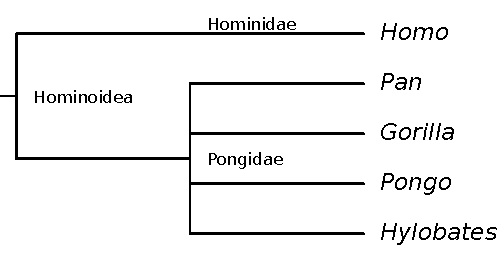
\includegraphics[scale=0.7]{homino_0.pdf} & 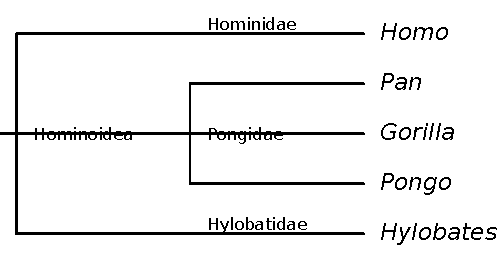
\includegraphics[scale=0.7]{homino_1.pdf} \\
3 (gibbons as outgroup) & 4 (Goodman, 1974: orangs as outgroup) \\
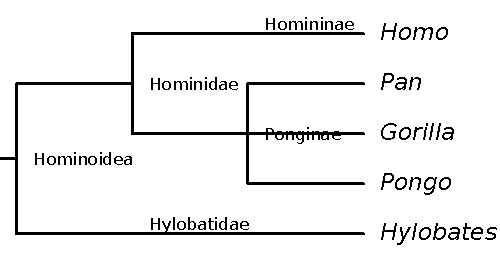
\includegraphics[scale=0.7]{homino_2.pdf} & 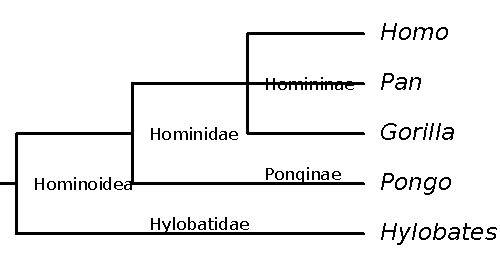
\includegraphics[scale=0.7]{homino_3.pdf} \\
5 (resolving trichotomy) & 6 (Goodman, 1990: gorillas as outgroup) \\
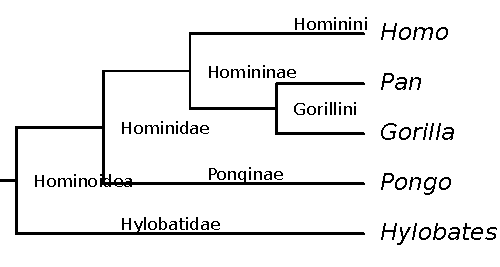
\includegraphics[scale=0.7]{homino_4.pdf} & 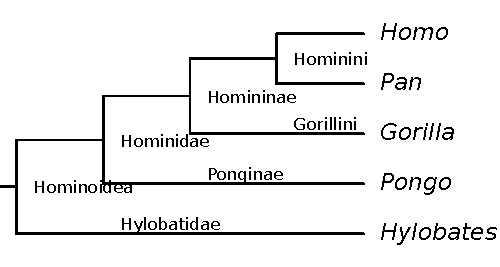
\includegraphics[scale=0.7]{homino_5.pdf} \\
7 (split of \emph{Hylobates}) \\
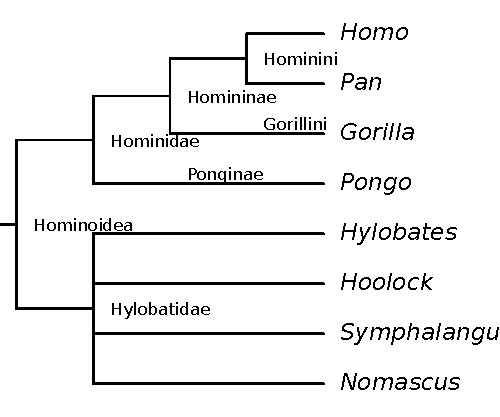
\includegraphics[scale=0.7]{homino_6.pdf} & 
\end{tabular}
\end{samepage}

\noindent{}Trees \#6 and \#7 match our criterion, the rest do not. To look for matching trees in \texttt{hominoidea.nw}, we pass the pattern on the command line:

\verbatiminput{match_1_txt.cmd}
\begin{samepage}
\verbatiminput{match_1_txt.out}
\end{samepage}

\noindent{}Note that only the pattern tree's topology matters: we would get the
same results with pattern \texttt{((Homo,Pan),Gorilla);},
\texttt{((Pan,Homo),Gorilla);}, etc., but not with
\texttt{((Gorilla,Pan),Homo);} (which would select trees \#1, 2, 3, and 5. In
future versions I might add an option for strict matching.

The behaviour of \match{} can be reversed by passing option \texttt{-v} (like
\texttt{grep -v}): it will print trees that \emph{do not} match the pattern.
Finally, note that \match{} only works on leaf labels (for now), and assumes
that labels are unique in both the pattern and the target tree.
